\chapter{Implementacja i eksperymenty}
Nasz program został zaimplementowany w języku C z wykorzystaniem biblioteki Nauty and Traces\cite{nauty}, która umożliwia łatwe obliczeniowo wykrywanie orbit, co znacznie przyspiesza proces generowania grafów. 
Autorem biblioteki nauty jest Brendan D. McKay, natomiast twórcą Traces jest Adolfo Piperno.

Jednym z aspektów powyższego kodu, który wykorzystujemy jest sposób przechowywania grafów w pamięci komputerowej, który bazuje na macierzy sąsiedztwa. Macierz sąsiedztwa to sposób reprezentacji grafu o N wierzchołkach przy użyciu macierzy kwadratowej o wymiarach NxN. Wartość na pozycji $(m, n)$ odpowiada  krawędzi pomiędzy wierzchołkami $m$ oraz $n$ (rysunek \ref{exmatrix}).
\begin{figure}[H]
  \centering
  \hfill
  \subfloat[]{
$\begin{bmatrix}
	0 & 1 & 0 & 0 & 1 \\
	1 & 0 & 0 & 0 & 1 \\
	0 & 0 & 0 & 0 & 1 \\
	0 & 0 & 0 & 0 & 0 \\
	1 & 1 & 1 & 0 & 0 \\
  \end{bmatrix}$
  }
  \hfill
  \subfloat[]{
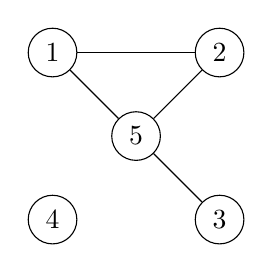
\begin{tikzpicture}[node distance={15mm}, main/.style = {draw, circle}, baseline=-8.0ex] 
    \node[main] (1) {$1$};
    \node[main] (2) [below right of=1] {$5$};
    \node[main] (3) [above right of=2] {$2$};
    \node[main] (4) [below left of=2] {$4$};
    \node[main] (5) [below right of=2] {$3$};

    \draw (1) -- (2);
    \draw (2) -- (3);

    \draw (2) -- (5);
    \draw (1) -- (3);
  \end{tikzpicture}
  }
  \hfill
  \hfill
  \caption{Graf wraz z odpowiadającą mu macierzą sąsiedztwa. W tej macierzy 0 odpowiada brakowi krawędzi, a 1 odpowiada jej istnieniu.}
  \label{exmatrix}
\end{figure}

Warto zauważyć nadmiarowość macierzy, gdzie każdej krawędzi w grafie odpowiadają dwie wartości. Ta nadmiarowość okazjonalnie pozwala na przyspieszenie obliczeń w zmodyfikowanej wersji macierzy sąsiedztwa używanej w naszym kodzie.
Modyfikacja metody macierzy sąsiedztwa polega na odejściu od zapisywania każdej liczby w macierzy jako liczby całkowitej. Jako że zajmujemy się jedynie grafami prostymi i niekolorowanymi, to wartości w poszczególnych komórkach mogą wynosić jedynie 0 lub 1. W związku z tym wiersz macierzy można zapisać nie jako $n$ wartości, a jako jedną liczbę całkowitą o odpowiedniej liczbie bitów. Ze względu na to, że największym grafem występującym w naszej pracy jest potencjalny graf 25 wierzchołkowy, 32 bitowa wartość jest wystarczająca żeby pomieścić wiersz macierzy reprezentujący wierzchołek dowolnego grafu który może zostać wygenerowany przez nasz program. 

Jedną ze znaczących prób optymalizacji które zostały podjęte były zmiany w algorytmie tworzenia przedziałów stożków prawdopodobnych. Algorytm sklejania jest bardzo wrażliwy na ich ilość ze względu na fakt, że operacja sklejania jest wykonywana dla każdej permutacji tych przedziałów po wierzchołkach grafu $G$. Początkowo, generacja była wykonana w sposób naiwny, gdzie kolejność rozbicia przedziału była zgodna z kolejnością wierzchołków w grafie. Takie podejście produkowało jednak zbyt wiele przedziałów, i z tego powodu zostało zmienione. Kolejnym algorytmem generującym przedziały był algorytm wzorujący się na algorytmie rozszerzania przedziałów. Kolejność rozbicia była w tym przypadku zależna od kolejności wykrycia klik $K_3$. Wynik tej metody wciąż nie był zadowalający, więc podjeliśmy ponowną próbę zmniejszenia liczby przedziałów. Tym razem opierała się ona na próbach ponownego połączenia przedziałów rozbitych we wcześniejszych krokach. Takie łączenie ponownie zmniejszyło ilość przedziałów. Łączenie zostało wykonane w sposób zachłanny, i nie ma gwarancji, że daje najlepszy możliwy zbiór przedziałów. Możliwe też, że dalsze modyfikacje algorytmu tworzącego zbiór przedziałów mogłyby przynieść lepszy wynik. Średnie ilości przedziałów dla każdej z metod ich tworzenia przedstawione zostały w tabeli \ref{tabPrzedzialy}

 \begin{table}[H]
 \begin{center}
 \begin{tabular}{|c c c c|} 
 \hline
 Rząd grafów & Pierwszy algorytm & Drugi algorytm & Drugi algorytm + łączenie \\ 
 \hline\hline
 17 & 2152 &  789 & 648\\
 \hline
 16 & 1470 & 521 & 401\\
 \hline
 15 & 175 & 84 & 74\\
 \hline
\end{tabular}
\end{center}
 \caption{Tabela porównująca średnią ilość przedziałów stworzonych dla zbiorów grafów o różnych rzędach}
 \label{tabPrzedzialy}
 \end{table}